\chapter{Derivatives and Rates of Change}

\section{Beginning Derivatives}

\subsection{Introduction}

One of the first concepts that you are introduced to in an algebra class is the concept of slope. When we have two points, \( \left( x_1, y_1 \right) \) and \( \left( x_2, y_2 \right) \), we can find a number that represents the "tilt" of line that passes through both of these points using the formula

\[ m = \dfrac{y_2 - y_1}{x_2 - x_1} \]

You may or may not have also learned that when we apply this formula to some function \( f \left( x \right) \), obtaining the slope between two points, it is called a \defterm{secant line}.

\begin{center}
    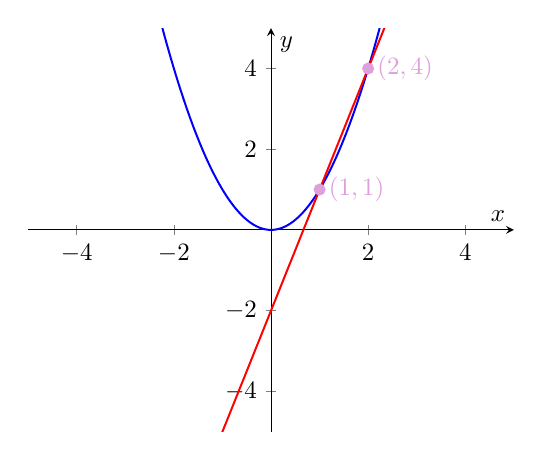
\begin{tikzpicture}[scale=.9]
        \begin{axis}[xmin=-5, xmax=5, xstep=1, ymin=-5, ymax=5, ystep=1, axis lines=middle, xlabel=\(x\), ylabel=\(y\), every axis plot/.append style={thick}]
            \addplot[color=blue, samples=100, smooth]{x^2};
            \addplot[color=red, samples=10]{3*x - 2};
            \addplot[color=Plum,mark=*] coordinates {(2, 4)} node[right, pos=1]{\( (2, 4) \)};
            \addplot[color=Plum,mark=*] coordinates {(1,1)} node[right, pos=1]{\( (1, 1) \)};
        \end{axis}
    \end{tikzpicture}
\end{center}

Let us now say that the distance between \( x_1 \) and \( x_2 \) is some value \( h \). Rewriting our terms, we can express this same secant slope using only a few variables.

\begin{align}
    m = \> &\dfrac{f \left( x + h \right) - f \left( x \right)}{\cancel{x} + h - \cancel{x}} \\
    = \> &\dfrac{f \left( x + h \right) - f \left( x \right)}{h}
\end{align}

This gives us the liberty of playing around with the values, \( h \) in particular. When \( h \) increases, the distance between the points increases, and generally the line looks nothing like the function. When we bring the two points together by making \( h \) some \textit{very} small value close to \( 0 \), though, something interesting happens. Our secant line with two points begins to look like a \defterm{tangent line} with only one point of intersection. In addition, the line begins to look much more similar to the function around the point.

\begin{center}
    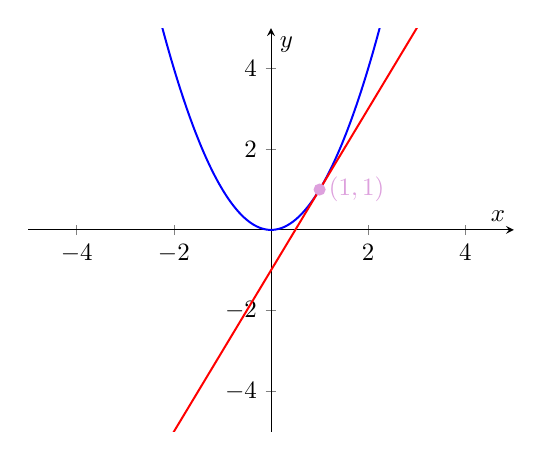
\begin{tikzpicture}[scale=.9]
        \begin{axis}[xmin=-5, xmax=5, xstep=1, ymin=-5, ymax=5, ystep=1, axis lines=middle, xlabel=\(x\), ylabel=\(y\), every axis plot/.append style={thick}]
            \addplot[color=blue, samples=100, smooth]{x^2};
            \addplot[color=red, samples=10]{2*x - 1};
            \addplot[color=Plum,mark=*] coordinates {(1,1)} node[right, pos=1]{\( (1, 1) \)};
        \end{axis}
    \end{tikzpicture}
\end{center}

This is interesting, but how do we express this very, almost infinitesimally, small value \( h \) mathematically? The answer is simple and is a concept that we have just learned. We need to take the limit as \( h \) approaches \( 0 \).

\begin{definition}{derivative}
    The \defterm{derivative} of a function \( f \) is the function \( f^\prime \) whose value at \( x \) is defined by
    \[ f^\prime \left( x \right) = \lim_{h \to 0} \dfrac{f \left( x + h \right) - f \left( x \right)}{h} \]
    The derivative represents the rate of change, or slope, at a specific point of the function \( f \).
\end{definition}

In addition, the alternative definition of the derivative at a point \( x = c \) is as follows.

\[ f^\prime \left( c \right) = \lim_{x \to c} \dfrac{f \left( x \right) - f \left( c \right)}{x - c} \]

where \( c \) will be a given real number. Only use this when directly specified.

\begin{notation}{derivative}
    Several derivative notations emerged throughout 1700-1800s and were used by various esteemed mathematicians of the time.
    
    \begin{multicols}{2}
    \begin{itemize}
        \item \( \dot y \) from Newton
        \item \( \dfrac{dy}{dx} = \dfrac{df}{dx} = \dfrac{d}{dx} \left( f \right) \) from Leibniz
        \item \( D_x \left( f \right) \) from Arbogast
        \item \( f^\prime \left( x \right) \) from Lagrange
    \end{itemize}
    \end{multicols}
    
    In addition, the partial derivative notation \( \frac{\partial}{\partial x} \) was pioneered by Legendre.
    
    There are also multiple ways of denoting \( n \)th derivatives, or the derivative applied \( n \) times.
    
    \begin{multicols}{2}
    \begin{itemize}
        \item \( \dfrac{d^n}{dx^n} \)
        \item \( y^{\prime \prime} \)
        \item \( f^{(n)} \left( x \right) \)
        \item \( y^{(n)} \left( x \right) \)
    \end{itemize}
    \end{multicols}
    
    While most of these notations are all somewhat relevant, the notations pioneered by Leibniz and Lagrange remain the most commonplace today.
\end{notation}

\begin{example}{derivative notation}
    \begin{align}
        y = x^2 &\implies y^\prime = 2x \\
        y = \sqrt{x} &\implies \dfrac{dy}{dx} = \dfrac{1}{2\sqrt{x}} \\
        y = \dfrac{1}{x} &\implies D_x \left( y \right) = -\dfrac{1}{x^2}
    \end{align}
\end{example}

Once we have a slope, obtained from evaluating the derivative of the function at the point, we can also find the tangent line itself.

\begin{definition}{tangent line}
    The tangent line to a function \( f \left( x \right) \) at a point \( x = a \) is given as follows
    
    \[ y - f \left( a \right) = f^\prime \left( a \right) \left( x - a \right) \]
    
    This represents a line with the same slope as the derivative at that point, intersecting at only one point.
\end{definition}

Although much more uncommon compared to the tangent slope, another related value is the \defterm{normal slope}.

\begin{definition}{normal slope/line}
    The \defterm{normal slope} of a function at a point \( x = a \) is the slope which is perpendicular to the tangent slope. This is expressed as
    
    \[ m_{\text{norm}} = -\dfrac{1}{m_{\text{tan}}} = -\dfrac{1}{f^\prime \left( a \right)} \]
    
    Just like with the tangent line, we can find the \defterm{normal line} to be

    \[ y - f \left( a \right) = -\frac{1}{f^\prime \left( a \right)} \left( x - a \right) \]
\end{definition}

\subsection{Differentiability}

Now that we know \textit{how} to find a derivative, we should also ask: \textit{When} can we find a derivative?

\begin{definition}{differentiable}
    We say that a function is \defterm{differentiable} at a point if we can find the derivative at that point. A function that is differentiable at every point of its domain is called a \defterm{differentiable function}. \par
    
    \vspace{0.3cm}
    
    \textbf{Note}: If a function is differentiable at a point, then it is also continuous at that point. This does \underline{not} imply that the converse, that a function that is continuous at a point is necessarily differentiable at the point, is true, however.
\end{definition}

\textbf{When is a function not differentiable?}

As a consequence of defining the derivative with limits, \textbf{continuity is a requirement for differentiability}. If a function is differentiable, it is also continuous. A function that is continuous, however, need not be differentiable. Consider the following cases.

\begin{itemize}
    \item Functions like \( y = \vert x \vert \) and other similar ones which have a sharp corner or a jump discontinuity in the slope will not have a derivative.
    \item At discontinuities and vertical asymptotes, either the limit or the function will not exist, meaning it will not be differentiable at that point.
    \item At completely vertical tangents, the slope will be infinite or undefined; therefore, the derivative will not exist.
    \item At cusps, which are similar to corners except that they are infinitely sharp, there will be an infinite discontinuity in the derivative, meaning it will not exist at that point.
\end{itemize}

\begin{example}{corner versus cusp}
    Corners and cusps may seem to be almost the same at first glance, but it is important to note their differences in order to differentiate between them.
    
    \vspace{0.3cm}
    
    The graph on the left shows the graph of \( f \left( x \right) = \vert x \vert \) (in {\color{blue} blue}), and its derivative (in {\color{red} red}). This is a \defterm{corner}. Notice the \textit{jump} discontinuity in the derivative.
    
    \vspace{0.3cm}
    
    The graph on the right shows the graph of \( f^\prime \left( x \right) = \sqrt[3]{x^2} \) (in {\color{blue} blue}), and its derivative (in {\color{red} red}). This is an example of a \defterm{cusp}. Notice the \textit{infinite} discontinuity.
    
    \begin{center}
    \begin{tikzpicture}[scale=0.7]
        \begin{axis}[xmin=-2, xmax=2, xstep=1, ymin=-2, ymax=2, ystep=1, axis lines=middle, xlabel=\(x\), ylabel=\(y\), every axis plot/.append style={thick}]
            \addplot[color=blue, samples=20, domain=-2:0]{-x};
            \addplot[color=blue, samples=20, domain=0:2]{x};
            \addplot[color=red, samples=10, domain=-2:0]{-1};
            \addplot[color=red, samples=10, domain=0:2]{1};
            \addplot[hole, color=red, fill=examplebg] coordinates{(0, -1)(0, 1)};
        \end{axis}
    \end{tikzpicture}
    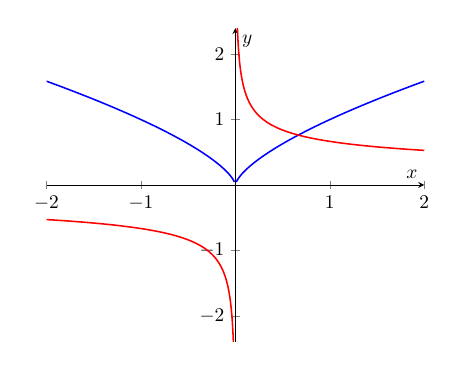
\begin{tikzpicture}[scale=0.7]
        \begin{axis}[xmin=-2, xmax=2, xstep=1, ymin=-2, ymax=2, ystep=1, axis lines=middle, xlabel=\(x\), ylabel=\(y\), enlarge y limits=true, restrict y to domain=-5:5, every axis plot/.append style={thick}]
            \addplot[color=blue, samples=200, smooth, domain=0.01:2]{pow(abs(x), 2/3)};
            \addplot[color=blue, samples=200, smooth, domain=-2:-0.01]{pow(abs(x), 2/3)};
            \addplot[color=red, samples=200, smooth, domain=0:2]{2 / (3 * pow(x, 1/3))};
            \addplot[color=red, samples=200, smooth, domain=-2:0]{2 / (3 * -pow(abs(x), 1/3))};
        \end{axis}
    \end{tikzpicture}
    \end{center}
\end{example}

\begin{example}{differentiable function}
    Consider the function \( f \left( x \right) \). Is it differentiable at \( x = 2 \)?
    \[
    f \left( x \right) = \begin{cases}
            3x - 2 & x < 2 \\
            x^2 & x \ge 2
        \end{cases}
    \]
    
    Using the left-hand limit definition of the derivative
    
    \begin{align}
        &\lim_{h \to 0^-} \dfrac{f \left( 2 + h \right) - f \left( 2 \right) }{h} \\
        = \> &\lim_{h \to 0^-} \dfrac{3 \left( 2 + h \right) - 2 - \left( 2 \right)^2}{h} \\
        = \> &\lim_{h \to 0^-} \dfrac{\cancel{6} + 3\cancel{h} - \cancel{2 - 4}}{\cancel{h}} \\
        = \> &3
    \end{align}
    
    Evaluating the right-hand limit
    
    \begin{align}
        &\lim_{h \to 0^+} \dfrac{f \left(2 + h \right) - f \left( 2 \right)}{h} \\
        = \> &\lim_{h \to 0^+} \dfrac{\left( 2 + h \right)^2 - 2^2}{h} \\
        = \> &\lim_{h \to 0^+} \dfrac{\cancel{2^2} + 4\cancel{h} + h^{\cancel{2}} - \cancel{2^2}}{\cancel{h}} \\
        = \> &4
    \end{align}
    
    Because the left-hand and the right-hand limits are not equal, the derivative does not exist; thus, the function \( f \) is not differentiable at \( x = 2 \).
\end{example}

\section{Derivatives with Calculators}

\subsection{Numeric Derivatives by Graph}

When encountering the terms CAS (computer algebra system) or NDER (numeric derivative), you will need to use a calculator to evaluate the derivatives. \par

Consider the function

\[ f \left( x \right) = \dfrac{2^{x + 1} - \sin{\left( \frac{x + 1}{x - 2} \right)}}{\sqrt[3]{x^3 - 2x + 7}} \]

To find the derivative using your calculator:

\begin{itemize}
    \item On a TI-84: Press \( 2 \)nd \( \to \) Press Trace \( \to \) Press \( \frac{dy}{dx} \)
    \item On a TI-89: Press F5 \( \to \) Press \( \frac{dy}{dx} \)
\end{itemize}

From there, you can use the point and the slope found to write the equation of a tangent line in point-slope form. Here's an example using the function \( f \) from earlier.

\[ y - 0.500 = 0.492 \left( x + 1 \right) \]

\begin{tip}
    Tangent lines can be left in point-slope form; there is no need to convert them to \( y = mx + b \) form on the test.
\end{tip}

For convenience, you can also use the equations that you've graphed as functions.

\begin{itemize}
    \item On a TI-84: Press the \verb+vars+ button \( \to \) Navigate to the heading \verb+Y-VARS+ \( \to \) Go to \verb+Function+ \( \to \) Press \( Y_1 \) (or the corresponding equation that you want the function for).
\end{itemize}

\subsection{Numeric Derivatives by Functions}

Given the function

\[ h \left( x \right) = \ln{\left( x \right)}\sin{\left( x \right)} \]

You may be prompted to find the derivative at some value, for example \( x = 3.2 \). While you can graph this function and find it like previously mentioned, a possibly faster way could be to use the derivative functions on the calculator.

\begin{itemize}
    \item On a TI-84: Go to \verb+math+ \( \to \) Press \verb+nDeriv+ \( \to \) Plug in the values and the variable that you are differentiating with respect to. For finding the derivative of \( h \left( x \right) \) at \( x = 3.2 \), it should look something like this:
    \[ \frac{d}{dx} \left( \ln{\left( x \right)} \sin{\left( x \right)} \right) \vert_{x=3.2} \]
    \item On a TI-89: Press F3 \( \to \) Press the \( d \) button \( \to \) Plug in the function \( \to \) Insert the vertical bar at the end of line and plug in the \( x \) value. For \( h \left( x \right) \) it would something like:
    \[ d \left( \ln{\left( x \right)} * \sin{\left( x \right)}, x \right) \vert_{x=3.2} \]
\end{itemize}

\subsection{Finding Second Derivatives}

Second derivatives are especially useful when finding things like acceleration.

\begin{itemize}
    \item On a TI-84: Nest the derivatives, setting the inner \( x \) equal to the outer \( x \). While a bit convoluted, it works:
    \[ \frac{d}{dx} \left( \frac{d}{dx} \left( \ln{\left( x \right)} \sin{\left( x \right)} \right) \vert_{x=x} \right) \vert_{x=3.2} \]
    \item On a TI-89: Simply add an extra argument to the derivative function with the degree (in this case: \( 2 \)):
    \[ d \left( \ln{\left( x \right)} * \sin{\left( x \right)}, x, 2 \right) \vert_{x=3.2} \]
\end{itemize}

\textbf{Note}: Those with a TI-89 also have the option of omitting the bar. This allows you to see the derivative function itself, which will be especially helpful later in Chapter 3 and Chapter 4.

\textbf{Note}: If you use another calculator type, such as the Nspire or a Casio, good luck :)

\subsection{Graphing Derivatives}

\begin{itemize}
    \item On a TI-84: Enter in the original function in the first equation entry, corresponding to \( y_1 \). From there, you can graph the derivative like usual, which should look like
    \[ \dfrac{d}{dx} \left( y_1 \right) \vert_{x=x} \]
    \item On a TI-89: This is quite similar to the TI-84. Graph the function in \( y_1 \) and then graph the derivative in \( y_2 \). It should look something like
    \[ d \left( y_1 \left( x \right), x \right) \]
\end{itemize}

\subsection{Deriving Numerical Derivatives}

\begin{definition}{Symmetric Difference Quotient}
    You will be asked to find the derivative in the same manner that your calculator finds the numerical derivative. This is the \defterm{Symmetric Difference Quotient}. The NDER function on your calculator uses a small, not infinitesimally though, value \( h \) with the formula
    
    \[ \dfrac{f \left( a + h \right) - f \left( a - h \right)}{2h} \]
    
    to calculate the slope at a point \( x = a \). Essentially, the calculator finds the slope of a secant line over a very small interval.
\end{definition}

If an \( h \) value is not specified in a question, it is assumed to be \( 0.01 \). In addition, there should not be a limit nor variables when using the SDQ.

\begin{example}{Symmetric Difference Quotient}
    Consider the function \( f \left( x \right) = x^2 \) at the point \( x = 3 \). Plugging in the information given, the Symmetric Difference Quotient will look something like
    
    \begin{align}
        &\dfrac{f \left( 3 + 0.01 \right) - f \left( 3 - 0.01 \right)}{2 \left( 0.01 \right)} \\
        = \> &\dfrac{\left( 3.01 \right)^2 - \left( 2.99 \right)^2}{0.02}
    \end{align}
    
    Utilizing the fact that this is a difference of squares
    
    \begin{align}
        &\dfrac{\cancel{\left( 3.01 - 2.99 \right)} \left( 3.01 + 2.99 \right)}{\cancel{0.02}} \\
        = \> &6
    \end{align}
\end{example}

\begin{example}{Symmetric Difference Quotient}
    Consider the function \( y = 3x - 2 \) at the point \( x = 4 \). Similarly to before, we can use the formula to get
    
    \begin{align}
        &\dfrac{f \left( 4.01 \right) - f \left( 3.99 \right)}{0.02} \\
        = \> &\dfrac{3 \left( 4.01 \right) - \cancel{2} - 3 \left( 3.99 \right) + \cancel{2}}{0.02} \\
        = \> &\dfrac{3 \cancel{\left( 4.01 - 3.99 \right)}}{\cancel{0.02}} \\
        = \> &3
    \end{align}
\end{example}

\subsection{Conclusion}

In summary, there are 5 different ways to find the derivative of a function at a point.

\begin{enumerate}
    \item Using the limit definition of the derivative.
    \item Using the alternative definition of the derivative.
    \item Using the NDER functions on your calculator.
    \item Using the grahping function on your calculator.
    \item Using the Symmetric Difference Quotient.
\end{enumerate}

\section{The Shortcuts}

Taking the limit or using the graphing function on your calculator to evaluate derivatives is not always convenient. In addition, you may want a simplified, closed-form function for the derivative. Luckily, there are shortcuts or rules that allow us to find derivatives algebraically.

\subsection{Rules}

\begin{rules}{Constant Rule}
    Because the graph of a constant line is horizontal, the slope is always \( 0 \). This is expressed as
    
    \[ y = k \implies y^\prime = 0, \quad k \in \mathbb{R} \]
\end{rules}

\begin{example}{Constant Rule}
    If \( y = 3 \), then \( y^\prime = 0 \).
\end{example}

\begin{rules}{Power Rule}
    For any function of the form \( y = x^n \), we can multiply the function by \( n \) and subtract \( 1 \) from the power. This is expressed as
    
    \[ y = x^n \implies y^\prime = nx^{n - 1} \]
\end{rules}

\begin{example}{Power Rule}
    For example,
    
    \begin{multicols}{2}
    \begin{itemize}
        \item \( \dfrac{d}{dx} \left( x^2 \right) = 2x \)
        \item \( \dfrac{d}{dx} \left( x^3 \right) = 3x^2 \)
        \item \( \dfrac{d}{dx} \left( 3x^3 \right) = 9x^2 \)
        \item \( \dfrac{d}{dx} \left( x^{100} \right) = 100x^{99} \)
    \end{itemize}
    \end{multicols}
    \vspace{0.1cm}
\end{example}

\begin{rules}{Constant Multiple Rule}
    If a function is multiplied by a constant number, then the derivative of the total function is equal to the constant times the function. This is expressed as
    
    \[ y = k f \left( x \right) \implies y^\prime = k f^\prime \left( x \right) \]
\end{rules}

\begin{example}{Constant Multiple Rule}
    For example, if \( y = 6x^2 \), then \( y^\prime = 6 \cdot 2x = 12 x \).
\end{example}

\begin{rules}{Sum and Difference Rule}
    The derivative of the sum of any number of terms is the same thing as the sum of the derivatives of the individual terms. This is expressed as
    
    \[ y = f \left( x \right) + g \left( x \right) \implies y^\prime = f^\prime \left( x \right) + g^\prime \left( x \right) \]
\end{rules}

\begin{example}{Sum and Difference Rule}
    For example, 
    \begin{align*}
        &\dfrac{d}{dx} \left( x^3 + x^2 + x + 1 \right) \\
        = \> &3x^2 + 2x + 1 + 0 \\
        = \> &3x^2 + 2x + 1
    \end{align*}
\end{example}

\begin{rules}{Product Rule}
    If you take the derivative of the product of two functions, it is equal to the first function times the derivative of the second function plus the second function times the derivative of the first function. This is written as
    
    \[ y = f \left( x \right) g \left( x \right) \implies y^\prime = f \left( x \right) g^\prime \left( x \right) + f^\prime \left( x \right) g \left( x \right) \]
\end{rules}

\begin{example}{Product Rule}
    For example, 
    \begin{align*}
        &\dfrac{d}{dx} \left( \left( x^2 \right) \left( 3x - 2 \right) \right) \\
        = \> &x^2 \left( 3 \right) + 2x \left( 3x - 2 \right) \\
        = \> &3x^2 + 6x^2 - 4x \\
        = \> &9x^2 - 4x
    \end{align*}
\end{example}

\begin{rules}{Quotient Rule}
    When given a rational function, the derivative works in a specific way.
    
    \[ y = \dfrac{f \left( x \right)}{g \left( x \right)} \implies y^\prime = \dfrac{f^\prime \left( x \right) g \left( x \right) - f \left( x \right) g^\prime \left( x \right)}{\left( g \left( x \right) \right)^2 } \]
    
    Note that, when applying the quotient rule, never expand out the denominator.
\end{rules}

\begin{example}{Quotient Rule}
    For an example, take
    
    \[ y = \dfrac{2x + 5}{3x^2 - 4} \]
    
    Then
    
    \begin{align*}
        y^\prime = \> &\dfrac{2 \left( 3x^2 - 4 \right) - 6x \left(2x + 5 \right)}{\left(3x^2 - 4 \right)^2} \\
        = \> &\dfrac{6x^2 - 8 - 12x^2 - 30x}{\left( 3x^2 - 4 \right)^2} \\
        = \> &\dfrac{-6x^2 - 30x - 8}{\left(3x^2 - 4 \right)^2} \\
        = \> &\dfrac{-2 \left(3x^2 + 15x + 4 \right)}{\left(3x^2 - 4 \right)^2}
    \end{align*}
\end{example}

\subsection{Second and Higher Order Derivatives}

Successive derivatives are generally straightforward. Apply differentiation multiple times.

Suppose \( y = x^6 - x^5 + 3x + 2 \), then

\begin{align}
    y^\prime = \> &6x^5 - 5x^4 + 3 \\
    \implies y^{\prime \prime} = \> &30x^4 - 20x^3 \\
    \implies y^{\prime \prime \prime} = \> &120x^3 - 60x^2 \\
    \implies y^{(iv)} = \> &360x^2 - 120x \\
    \implies y^{(v)} = \> &720x - 120 \\
    \implies y^{(vi)} = \> &720 \\
    \implies y^{(vii)} = \> &0 \\
    \implies y^{(viii)} = \> &0 \\
    \vdots
\end{align}

Note that when taking derivatives higher than order three, the prime (\(^\prime\)) symbols in the exponent change to roman numerals.

Also note that we can, theoretically, infinitely differentiate this, which will always evaluate to \( 0 \). This means that there are infinite derivatives of the function.

\begin{tip}
    If, when asked to find \textit{all} derivatives, you list only the first \( n \), you will get \textbf{0 points}. You need to list a general form for the higher order derivatives. In addition to derivatives \( y^\prime \) through \( y^{(vi)} \) above, you will need to write
    
    \[ y^{(n)} = 0, \text{for all } n \ge 7 \]
\end{tip}

\subsection{Finding Horizontal Tangents}

The slope of a horizontal line is always \( 0 \). In addition, the derivative of a function represents the slope of a line. So, in order to find a horizontal tangent, set the derivative of a line to 0.

\begin{example}{Finding a Horizontal Tangent}
    Consider the function \( y = x^2 - 8x + 5 \). Its derivative is the function \( y^\prime = 2x - 8 \). Setting this to 0, we get
    
    \begin{align}
        0 &= 2x - 8 \\
        8 &= 2x \\
        x &= 4
    \end{align}
    
    So the function has a horizontal tangent at \( x = 4 \). If you are asked to find the \textit{point} at which the tangent line is horizontal, plug the found \( x \) value back into the \textbf{original} function, not the derivative. \( 4^2 - 8 \left( 4 \right) + 5 = -11 \), so the point at which there is a horizontal tangent is \( \left(4, -11 \right) \).
\end{example}

\section{Velocity, Acceleration, and Other Derivatives}

When given a function that represents a position or a cost at a specific time or unit, its derivatives have special connotations.

\subsection{Introduction}

The position of an object at a time is usually denoted by some function \( s \left( t \right) \), where \( t \) represents time.

\begin{definition}{velocity}
    \defterm{Velocity}, usually referring to instantaneous velocity, is the \textit{first derivative} of the position function.

    \[ s^\prime \left( t \right) = v \left( t \right) \] 

    In addition, when the velocity changes sign (passes through the \( x \)-axis and goes forward), the direction of the object moving at that velocity changes.
\end{definition}

\begin{example}{velocity}
For example, given the position function \( s \left( t \right) = t^2 \), the velocity function is \( v \left( t \right) = s^\prime \left( t \right) = 2t \).
\end{example}

\begin{definition}{speed}
    Another key term is \defterm{speed}, which is velocity without direction, is defined as

    \[ \text{speed} = \vert v \left( t \right) \vert \]
\end{definition}

\begin{example}{speed}
    For example, if \( v \left( a \right) = -2 \) for some point \( a \), then the speed at that point \( a \) is \( 2 \) units.
\end{example}

\begin{definition}{acceleration}
    \defterm{Acceleration} is the rate of change of velocity, so it is the first derivative of velocity, meaning that it is also the second derivative of position.

    \[ a \left( t \right) = v^\prime \left( t \right) = s^{\prime \prime} \left( t \right) \]
\end{definition}

\begin{example}{acceleration}
    Using the function \( s \left( t \right) = t^2 \) from earlier, \( a \left( t \right) = v^\prime \left( t \right) = 2 \).
\end{example}

While this is not really necessary knowledge, the derivative of acceleration (and thus the third derivative of position) is called \defterm{jerk}, which sounds somewhat funny.

\subsection{Problems Utilizing Derivatives}

\begin{itemize}
    \item \textbf{How do you find the time at which a particle reaches its maximum height given a position function \( s \left( t \right) \)?} If we try visualizing a graph with a maximum and its derivative, it is apparent that, at the maximum, the derivative is equal to \( 0 \). So, in order to solve for the \( t \) at which the function is at its maximum, set the derivative of the position function (the velocity) equal to \( 0 \) and solve for \( t \). Note that this also works for minimums.

    \item \textbf{How do you find a particle's position at the maximum height?} After acquiring the time using the previously mentioned method, you can plug it into the \textit{original} function.

    \item \textbf{How do you find out how long a particle has been in the air?} For this, you can either multiply the time at which the particle is at its maximum by \( 2 \) or find the distance between the two zeroes of the original function.
\end{itemize}

\subsection{Cost and Revenue}

Another common application of derivatives is with cost functions.

The average increase of cost is synonymous with the average rate of change. Given a cost function \( c \left( x \right) \), where \( x \) represents units produced, the average increase of cost is

\[ \dfrac{\Delta c}{\Delta x} \]

\begin{definition}{marginal cost}
    \defterm{Marginal cost} is the estimate of the cost of producing one more unit. To find marginal cost, evaluate the derivative of the cost function at the current \( x \) value.

    \[ \text{Marginal cost} = c^\prime \left( x \right) \]
\end{definition}

\begin{example}{marginal cost}
    For example, suppose that it costs
    
    \[ c \left( x \right) = x^3 - 6x^2 + 15x + 100 \]
    
    to produce \( x \) stoves and you currently make \( 10 \) stoves per day. The marginal cost of producing one more unit would be
    
    \[ c^\prime \left( 10 \right) = 3 \left( 10 \right)^2  - 12 \left( 10 \right) + 15 = 300 - 120 + 15 = 195 \]
    
    Thus, the estimated cost for producing one more stove would be \$195.
\end{example}

Also recalling that revenue is the cost subtracted from the total, or gross, income,

\begin{definition}{marginal revenue}
    \defterm{Marginal revenue} works similarly to marginal cost and is the estimated revenue for producing one more unit. To find it, take the derivative of a revenue function and evaluate it at the point \( x \).

    \[ \text{Marginal revenue} = r^\prime \left( x \right) \]
\end{definition}

\section{Derivatives of Trig Functions}

This section tackles the derivatives of trigonometric functions. Suppose we wanted to find the derivative of a function such as \( y = \sin{x} \).

Using the limit definition,

\begin{align}
    &\lim_{h \to 0} \dfrac{\sin{\left( x + h \right)} - \sin{\left( x \right)}}{h} \\
    = \> &\lim_{h \to 0} \dfrac{\sin{x}\cos{h} + \sin{h}\cos{x} - \sin{x}}{h} \\
    = \> &\lim_{h \to 0} \dfrac{\sin{x} \left( \cos{h} - 1 \right) + \sin{h}\cos{x}}{h} \\
    = \> &\lim_{h \to 0} \dfrac{\sin{x} \left( \cos{h} - 1 \right)}{h} + \lim_{h \to 0} \dfrac{\cancel{\sin{h}} \cos{x}}{\cancel{h}} \\
    = \> &\cancelto{0}{\lim_{h \to 0} \dfrac{-\sin{x}\sin^2{h}}{h \left( \cos{h} + 1 \right)}} + \cos{x} \\
    = \> &\cos{x}
\end{align}

Thus,

\[ \dfrac{d}{dx} \left( \sin{x} \right) = \cos{x} \]

Of course, this is quite cumbersome, so it is recommended to know the trigonometric derivatives by definition.

Similarly to \( \sin{x} \),

\[ \dfrac{d}{dx} \left( \cos{x} \right) = -\sin{x} \]

Now that we have the derivatives of the two fundamental trigonometric functions, we can define the others in terms of them and find their derivatives.

For \( y = \tan{x} \), we can use the quotient rule to get

\begin{align}
    &\dfrac{d}{dx} \left( \dfrac{\sin{x}}{\cos{x}} \right) \\
    = \> &\dfrac{\cos^2{x} + \sin^2{x}}{\cos^2{x}} \\
    = \> &\dfrac{1}{\cos^2{x}} \\
    = \> &\sec^2{x}
\end{align}

For the other three trig functions, similar methods can be used to find the derivatives.

\begin{definition}{trig derivatives}
    
    In total, you need to have these six key trig derivatives memorized.
    
    \begin{multicols}{2}
    \begin{itemize}
        \item \( \dfrac{d}{dx} \left( \sin{x} \right) = \cos{x} \)
        \item \( \dfrac{d}{dx} \left( \cos{x} \right) = -\sin{x} \)
        \item \( \dfrac{d}{dx} \left( \tan{x} \right) = \sec^2{x} \)
        \item \( \dfrac{d}{dx} \left( \csc{x} \right) = -\csc{x}\cot{x} \)
        \item \( \dfrac{d}{dx} \left( \sec{x} \right) = \sec{x}\tan{x} \)
        \item \( \dfrac{d}{dx} \left( \cot{x} \right) = -\csc^2{x} \)
    \end{itemize}
    \end{multicols}
    
    \vspace{0.1cm}
    
\end{definition}

\begin{tip}
    It is sometimes helpful to simplify expressions first by using trigonometric identities before taking the derivative.
    
    Consider the function
    
    \[ y = \cos{x}\sec{x} \]
    
    Although we could use the product rule to find the derivative, a far easier solution is to realize that
    
    \begin{align}
        y = &\cos{x}\sec{x} \\
        = \> &\cancel{\cos{x}} \cdot \dfrac{1}{\cancel{\cos{x}}} \\
        = \> &1
    \end{align}
    
    Then, taking the derivative of a constant,
    
    \[ y^\prime = 0 \]
\end{tip}